\documentclass[a4paper,leqno,twocolumn]{article}
% ==== Inputs and Usepackages ====

\usepackage{tablefootnote}
\usepackage{enumerate}
\usepackage{float}
\usepackage{url}
\usepackage{hyperref}
\usepackage{dsfont}
\usepackage{mathrsfs}
\usepackage{amsmath}
\usepackage{amssymb}
\usepackage{amsthm}
\usepackage{amsfonts}
\usepackage{mathtools}
%\usepackage{mathabx}
\usepackage{MnSymbol}
\usepackage{xfrac}
\usepackage{nicefrac}
\usepackage{geometry}
\usepackage{graphicx}
\usepackage{graphics}
\usepackage{latexsym}
\usepackage{setspace}
\usepackage{tikz-cd}
\usepackage{tikz}
 \usetikzlibrary{matrix}
 \usetikzlibrary{calc}
 \usetikzlibrary{circuits.ee.IEC}
\usepackage{circuitikz}

\usepackage{a4wide}
\usepackage{fancybox}
\usepackage{fancyhdr}
\usepackage[utf8]{inputenc}




% ==== Page Settings ====

\hoffset = -1.2 in
\voffset = -0.3 in
\textwidth = 590pt
\textheight = 770pt
\setlength{\headheight}{20pt}
\setlength{\headwidth}{590pt}
\marginparwidth = 0 pt
\topmargin = -0.75 in
\setlength{\parindent}{0cm}


% ==== Presettings for files ====

\pagestyle{fancy}


\cfoot{\thepage}
\lfoot{\href{mailto:szekerb@student.ethz.ch}{szekerb@student.ethz.ch}}
\rfoot{Balázs Szekér, \today}
\lhead{Physics \uproman{3} Summary}

% ==== General Commands ====

\newcommand{\sframebox}[1]{
        \framebox[500pt][l]{\parbox{490pt}{
            #1
        }
    }

}

\newcommand{\cframebox}[2]{
        \fbox{\parbox{#1pt}{
            #2
        }
    }
}









% ====== Maths ======


% ==== Formats ====
\newcommand{\boldline}[1]{\textbf{\underline{#1}}}
\newcommand{\uproman}[1]{\uppercase\expandafter{\romannumeral#1}}
\newcommand{\lowroman}[1]{\romannumeral#1\relax}
\newcommand{\fat}[1]{\textbf{#1}}
\newcommand{\Loesung}{\begin{center}\textbf{Lösung}\end{center}}

\newcommand{\Korollar}[1]{\textbf{Korollar} \vspace{1\baselineskip} #1}
\newcommand{\Beispiel}[1]{\textbf{Beispiel} \vspace{1\baselineskip} #1}
\newcommand{\Beweis}[1]{\textbf{Beweis} \vspace{1\baselineskip} #1}
\newcommand{\Proposition}[1]{\textbf{Proposition} \vspace{1\baselineskip} #1}
\newcommand{\Satz}[1]{\textbf{Satz} \vspace{1\baselineskip} #1}
\newcommand{\Definition}[1]{\textbf{Definition} \vspace{1\baselineskip} #1}
\newcommand{\Lemma}[1]{\textbf{Lemma}\vspace{1\baselineskip} #1}
\newcommand{\Bemerkung}[1]{\textbf{Bemerkung} \vspace{1\baselineskip} #1}
\newcommand{\Theorem}[1]{\textbf{Theorem} \vspace{1\baselineskip} #1}




% ==== mathsymbols ====
\newcommand{\Q}{\mathbb{Q}}
\newcommand{\R}{\mathbb{R}}
\newcommand{\N}{\mathbb{N}}
\newcommand{\Z}{\mathbb{Z}}
\newcommand{\C}{\mathbb{C}}
\newcommand{\K}{\mathbb{K}}
\newcommand{\eS}{\mathbb{S}}
\newcommand{\X}{$X$ }
\newcommand{\Y}{$Y$ }
\newcommand{\x}{$x$ }
\newcommand{\y}{$y$ }
\newcommand{\B}{\mathcal{B}}
\newcommand{\A}{\mathcal{A}}
\renewcommand{\S}{\mathcal{S}}
\renewcommand{\P}{\mathcal{P}}



% ==== math operators ====
\newcommand{\klammer}[1]{\left( #1 \right)} 
\newcommand{\eckigeklammer}[1]{\left[ #1 \right]}
\newcommand{\geschwungeneklammer}[1]{\left\{ #1 \right\}}
\newcommand{\floor}[1]{\left\lfloor #1 \right\rfloor}
\newcommand{\ceil}[1]{\left\lceil #1 \right\rceil}
\newcommand{\scalprod}[2]{\left\langle #1 , #2 \right\rangle}
\newcommand{\abs}[1]{\left\vert #1 \right\vert} 
\newcommand{\Norm}[1]{\left\vert\left\vert #1 \right\vert\right\vert}
\newcommand{\intab}{\int_a^b}
\newcommand{\intii}{\int_{-\infty}^\infty} 
\newcommand{\cint}[2]{\int_{#1}^{#2}}
\newcommand{\csum}[2]{\sum_{#1}^{#2}}
\newcommand{\limes}[1]{\lim\limits_{#1}}
\newcommand{\limessup}[1]{\limsup\limits_{#1}}
\newcommand{\limesinf}[1]{\liminf\limits_{#1}}
\newcommand{\limesninf}{\limes{n \rightarrow \infty}}
\newcommand{\limsupninf}{\limessup{n \rightarrow \infty}}
\newcommand{\liminfninf}{\limesinf{n \rightarrow \infty}}
\newcommand{\standardNorm}{\Norm{ \ \cdot \ }}
\newcommand{\einsNorm}{\Norm{ \ \cdot \ }_1}
\newcommand{\zweiNorm}{\Norm{ \ \cdot \ }_2}
\newcommand{\Hom}{\text{Hom}}
\newcommand{\Mat}{\text{Mat}}
\newcommand{\grad}{\text{grad}}
\newcommand{\vol}{\text{vol}}
\newcommand{\supp}{\text{supp}}
\newcommand{\rot}{\text{rot}}
\renewcommand{\div}{\text{div}}



% ==== Analysis ====
\newcommand{\supremum}{\text{sup}}
\newcommand{\infimum}{\text{inf}}
\newcommand{\maximum}{\text{max}}
\newcommand{\minimum}{\text{min}}

\newcommand{\xinX}{$x \in X$ }
\newcommand{\yinY}{$y \in Y$ }
\newcommand{\xyinX}{$x,y \in X$ }
\newcommand{\yinX}{$y \in X$ }
\newcommand{\xinR}{$x \in \R$ }
\newcommand{\xyinR}{$x,y \in \R$ }
\newcommand{\zinC}{$z \in \C$ }
\newcommand{\ninN}{$n \in \N$ }
\newcommand{\NinN}{$N \in \N$}
\newcommand{\angeordneterK}{$(K,\leq)$ }
\newcommand{\xFolge}{(x_n)_{n=0}^{\infty}}
\newcommand{\yFolge}{(y_n)_{n=0}^{\infty}}
\newcommand{\zFolge}{(z_n)_{n=0}^{\infty}}
\newcommand{\aFolge}{(a_n)_{n=0}^{\infty}}
\newcommand{\fFolge}{(f_n)_{n=0}^{\infty}}

\newcommand{\XsubR}{$X \subset \R$ }
\newcommand{\XsubeqR}{$X \subseteq \R$ }

\newcommand{\XFam}{\mathcal{X}}
\newcommand{\PFam}{\mathcal{P}}

\newcommand{\offenesintervall}[2]{$\left( #1 , #2 \right)$ }
\newcommand{\abgeschlossenesintervall}[2]{$\left( #1 , #2 \right)$ }

\newcommand{\XTopRaum}{(X,\tau)}


% ==== Lineare Algebra ====
\newcommand{\vinV}{$v \in V$ }
\newcommand{\uinU}{$u \in U$ }
\newcommand{\winW}{$w \in W$ }
\newcommand{\vwinV}{$v,w \in V$ }

\newcommand{\BasisV}{v_1 , \dots , v_n}
\newcommand{\BasisU}{u_1 , \dots , u_n}
\newcommand{\BasisW}{w_1 , \dots , w_n}

\newcommand{\transpose}[1]{#1^t}
\newcommand{\inverse}[1]{#1^{-1}}
\newcommand{\ddvec}[3]{\left( #1,#2,#3 \right)}
\newcommand{\tdvec}[2]{\left( #1 , #2 \right)}

\newcommand{\Edrei}{\begin{pmatrix}
    1 & 0 & 0 \\
    0 & 1 & 0 \\
    0 & 0 & 1
\end{pmatrix}}

\newcommand{\id}{\text{id}}
\newcommand{\GL}{\text{GL}}
\newcommand{\End}{\text{End}}
\renewcommand{\Im}{\text{Im}}
\renewcommand{\Re}{\text{Re}}
\renewcommand{\ker}{\text{Ker}}
\newcommand{\rang}{\text{rang}}
\newcommand{\ad}{\text{ad}}
\newcommand{\Eig}{\text{Eig}}
\newcommand{\Bil}{\text{Bil}}
\newcommand{\sign}{\text{sign}}
\newcommand{\tr}{\text{tr}}



% ====== Physics ======

% ==== Physicssymbols ====
\newcommand{\epsilonnull}{\epsilon_0}
\newcommand{\munull}{\mu_0}
\newcommand{\rn}{r_0}
\newcommand{\Rn}{R_0}
\newcommand{\rhonull}{\rho_0}
\newcommand{\Rhonull}{\varrho_0}


% ==== Notation ====
\newcommand{\Etot}{E_{\text{Tot}}}
\newcommand{\Wtot}{W_{\text{Tot}}}
\newcommand{\Ftot}{F_{\text{Tot}}}
\newcommand{\vtot}{v_{\text{Tot}}}
\newcommand{\atot}{a_{\text{Tot}}}
\newcommand{\mtot}{m_{\text{Tot}}}
\newcommand{\Mtot}{M_{\text{Tot}}}

\newcommand{\Ekin}{E_{\text{Kin}}}
\newcommand{\Epot}{E_{\text{Pot}}}
\newcommand{\Edef}{E_{\text{Def}}}

\newcommand{\Fg}{F_g}
\newcommand{\FN}{F_N}
\newcommand{\Fz}{F_z}
\newcommand{\FC}{F_C}

\newcommand{\xn}{x_0}
\newcommand{\xN}{x_n}
\newcommand{\vn}{v_0}
\newcommand{\vN}{v_n}
\newcommand{\an}{a_0}
\newcommand{\aN}{a_n}

\newcommand{\dt}{\Delta t}
\newcommand{\dx}{\Delta x}
\newcommand{\dv}{\Delta v}
\newcommand{\da}{\Delta a}
\newcommand{\dE}{\Delta E}
\newcommand{\dW}{\Delta W}
\newcommand{\dF}{\Delta F}


% ==== Relativity ====
\newcommand{\relsqrt}{\sqrt{1-\frac{v^2}{c^2}}}
\newcommand{\relgamma}{\frac{1}{\relsqrt}}


% ==== Constants ====
\newcommand{\g}{9.81}




\raggedbottom

\renewcommand*{\figurename}{Abb.}
\renewcommand{\epsilon}{\varepsilon}
\clubpenalty = 10000
\widowpenalty = 10000

\theoremstyle{definition}
\newtheorem*{theorem}{Theorem}
\newtheorem*{definition}{Definition}
\newtheorem*{lemma}{Lemma}
\newtheorem*{proposition}{Proposition}
\newtheorem*{beispiel}{Beispiel}
\newtheorem*{korollar}{Korollar}
\newtheorem*{bemerkung}{Bemerkung}
\newtheorem*{beweis}{Beweis}

%\setcounter{section}{-1}

\begin{document}

\section{Multiple Linear Regression}

Model Formula and assumptions: $Y_i = \sum_{j=1}^p \beta_j x_{ij} + \epsilon_i \ \Leftrightarrow \ Y = X \beta + \epsilon \ \Leftrightarrow \ Y_i = x_i^T \beta + \epsilon_i \ \Leftrightarrow \ Y_i = \beta_1 + \sum_{j=2}^p X_{ij} \beta_j + \epsilon_i$ where $\epsilon_1,\dots,\epsilon_n \stackrel{\text{iid}}{\sim} \mathcal{N}(0,\sigma^2)$ hence $\Cov(\epsilon) = \sigma^2 \id$. Assume $n \geq p$ and thus $X$ has full rank.

\vspace{4pt}

\fat{Least Squares Model}
$\hat{\beta} = \argmin \Norm{Y - X \beta}_2^2 = (X^T X)^{-1} X^T Y$. Def: $\epsilon_i \approx Y_i - x_i^T \beta := r_i \ \Rightarrow \ \hat{\sigma}^2 = \frac{1}{n-p} \sum_{i=1}^n r_i^2$.

\vspace{4pt}

\fat{Assumptions:} 1) LinRegEq is correct ($\Expec \eckigeklammer{\epsilon_i} = 0$), 2) $x_i$'s are exact, 3) Var of Errors is const ($\Var(\epsilon_i) = \sigma^2$) ("Homoscedasticity"), 4) Errors are uncorrelated ($\Cov(\epsilon_i,\epsilon_j) = 0$), 5) Errors $\epsilon_i$ are jointly normally distributed $\Rightarrow$ $Y_i$'s are jointly normally distributed.

\vspace{4pt}

\fat{Geometric Interpretation}
$X \hat{\beta}$ is the orthogonal projection of $Y$ onto $\mathcal{X} \equiv$ span$(X)$ (columnwise span) $\Rightarrow \ \hat{Y} = X \hat{\beta} = \underbrace{X (X^T X)^{-1} X^T}_{:= P} Y$. $\mathcal{X}$ is a $p$-dim subspace of $\R^n$, $P = P^T = P^2$, $\tr(P) = \tr(\id_p) = p$. The residuals live in $\mathcal{X}^\perp$: $\vec{r} = (1-P) \vec{Y}$.

%\paragraph{Estimating $\beta_j$'s:} $H_{0,j}: \ \beta_j = 0$, std.error: $\sqrt{\widehat{\Var}(\hat{\beta}_j)}$

\vspace{-5pt}

\subsection{Properties of LS Estimator}
(i) $\Expec\eckigeklammer{\hat{\beta}} = \beta$ hence $\hat{\beta}$ is an unbiased estimator,
(ii) $\Expec\eckigeklammer{\hat{Y}} = \Expec\eckigeklammer{Y} = X \beta$, $\Expec\eckigeklammer{r} =0$,
(iii) $\Cov(\hat{\beta}) = \sigma^2 \klammer{X^T X}^{-1}$,
(iv) $\Cov(\hat{Y}) = \sigma^2 P$, $\Cov(r) = \sigma^2 (1-P)$,
(v) $\Var(r_i) = \sigma^2 (1-P_{ii})$ hence $\Expec\eckigeklammer{\sum_i r_i^2} = \sum_i \Var(r_i) = \sigma^2 (n-\tr(P)) = \sigma^2 (n-p)$ hence $\Expec\eckigeklammer{\hat{\sigma}} = \Expec\eckigeklammer{\frac{1}{n-p} \sum_i r_i^2} = \sigma$ hence an unbiased estimator,
(vi) $\hat{\beta} \sim \mathcal{N}_p \klammer{\beta,\sigma^2 \klammer{X^T X}^{-1}}$, $\hat{Y} \sim \mathcal{N}_n \klammer{X \beta,\sigma^2 P}$, $r \sim \mathcal{N}_n \klammer{0,\sigma^2 (1-P)}$, $\hat{\sigma}^2 \sim \frac{\sigma^2}{n-p} \chi_{n-p}^2$

\vspace{-5pt}

\subsection{Tests and Confidence Regions}
$H_{0,j}: \ \beta_j = 0$, std.error: $\sqrt{\widehat{\Var}(\hat{\beta}_j)}$. Thus: $\frac{\hat{\beta}_j}{\sqrt{\sigma^2 (X^T X)_{jj}^{-1}}} \sim \mathcal{N}(0,1)$ under $H_{0,j}$ and $T_j = \frac{\hat{\beta}_j}{\sqrt{\hat{\sigma}^2 \klammer{X^T X}_{jj}^{-1}}} \sim t_{n-p}$ under $H_{0,j}$. Conf Int: $\hat{\beta}_j \pm \sqrt{\hat{\sigma}^2 \klammer{X^T X}_{jj}^{-1}} \cdot t_{n-p;1-\frac{\alpha}{2}}$

\vspace{4pt}

\fat{Test of global $H_0$}
$H_0$: $\beta_2 = \dots = \beta_p = 0$, $H_A$: $\exists j \in \geschwungeneklammer{2,\dots,p}: \beta_j \neq 0$.
$F = \frac{\Norm{\hat{Y} - \bar{Y}}_2^2 / (p-1)}{\Norm{Y - \hat{Y}}_2^2 / (n-p)} \sim F_{p-1,n-p}$ under $H_0$.
$R^2 = \frac{\Norm{\hat{Y} - \bar{Y}}_2^2}{\Norm{Y - \hat{Y}}_2^2} = 1 - \frac{\Norm{Y - \hat{Y}}_2^2}{\Norm{Y-\bar{Y}}_2^2}$

\vspace{4pt}

\fat{Confidence Lvls} We say a Test $T_n : \mathcal{X}^n \rightarrow \geschwungeneklammer{0,1}$ is (i) lvl $\alpha$ if: $\sup_{P \in H_0} \mathbb{P}_{P^n} (T_n = 1) \leq \alpha$, (ii) pointwise asymptotic lvl $\alpha$ if $\sup_{P \in H_0} \lim_{n \rightarrow \infty} \mathbb{P}_{P^n} (T_n = 1) \leq \alpha$, (iii) uniform asymptotic lvl $\alpha$ if $\lim_{n \rightarrow \infty} \sup_{P \in H_0} \mathbb{P}_{P^n} (T_n = 1) \leq \alpha$

\vspace{4pt}

\fat{p-value} Infimum over all significance lvl's $\alpha$ s.t. test rejects.

\vspace{4pt}

\fat{For new $x_0$:}
Confidence Interval: $\frac{x_0^T \hat{\beta} - x_0^T \beta}{\hat{\sigma} \sqrt{x_0^T \klammer{X^T X}^{-1} x_0}} \sim t_{n-p}$,

Prediction Interval: $\frac{y_0 - x_0^T \hat{\beta}}{\hat{\sigma} \sqrt{1 + x_0^T \klammer{X^T X}^{-1} x_0}} \sim t_{n-p}$

\vspace{-5pt}

\subsection{Analysis of Residuals \& Checking of Model Assumptions}

\vspace{-5pt}

\paragraph{Tukey-Anscombe Plot} Plot $r_i$ vs. $\hat{Y}_i$'s.

\vspace{2pt}

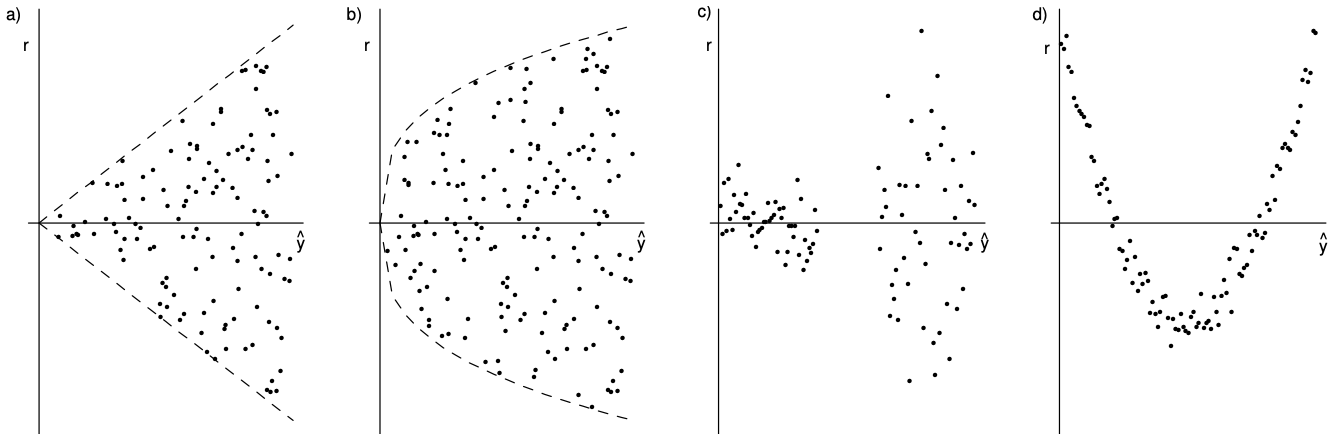
\includegraphics[width=0.49\textwidth]{Bilder/TukeyAnscombe.png}

\vspace{1pt}

a) Linear increase of sd (solution: log-transform), b) non-linear increase of sd, c) 2 groups with different variances, d) missing quadratic term in the model

\vspace{-5pt}

\paragraph{QQ-Plot} Plot empirical quantiles vs. theoretical quantiles of $\mathcal{N}(0,1)$. If $r \sim \mathcal{N}(\mu,\sigma^2)$, then plot would be a straight line.

\vspace{1pt}

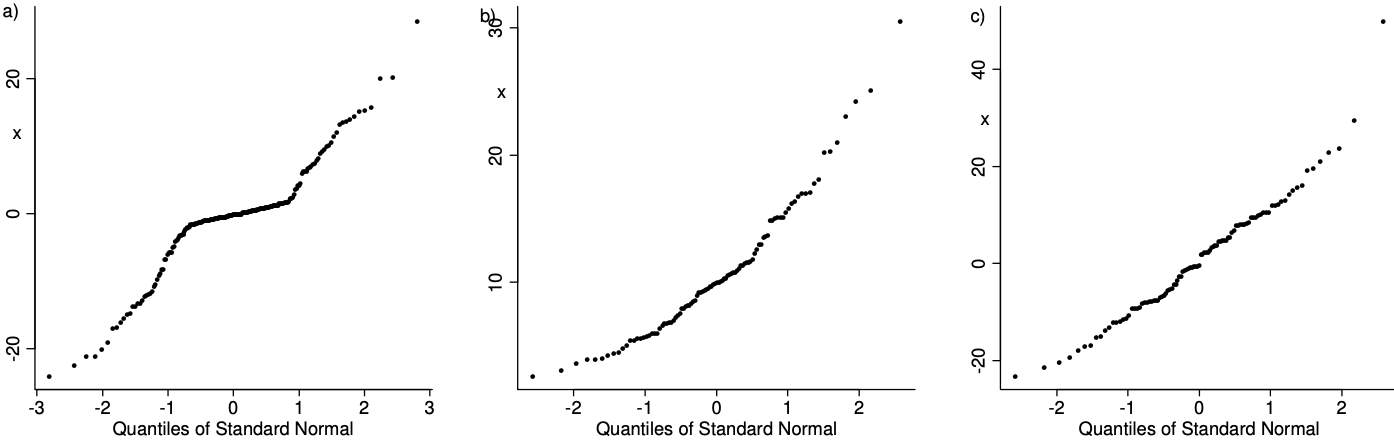
\includegraphics[width=0.4\textwidth]{Bilder/QQPlot.png}

\vspace{1pt}

a) long-tailed distribution, b) skewed distribution, c) dataset with outlier

\subsection{Generalized LS and weighted Regression}
$Y = X \beta + \epsilon$, $\epsilon \sim \mathcal{N}_n(0,\SigmaCov)$, $\SigmaCov$ known and $\SigmaCov = C C^T$. Reformulate: $\tilde{Y} = \tilde{X} \beta + \tilde{\epsilon}$ with $\tilde{Y} = C^{-1} Y$, $\tilde{X} = C^{-1} X$, $\tilde{\epsilon} \sim \mathcal{N}_n (0,\id)$ and obtain: $\hat{\beta} = \klammer{X^T \SigmaCov^{-1} X}^{-1} X^T \SigmaCov^{-1} Y$, $\Cov(\hat{\beta}) = \klammer{X^T \SigmaCov^{-1} X}^{-1}$

\vspace{1pt}

Special Case: $\SigmaCov = \sigma^2 \text{diag}(z_1,\dots,z_n)$ $\Rightarrow$ weighted LS problem: $\min_\beta \sum_{i=1}^n w_i \klammer{Y_i - x_i^T \beta}$, $w_i = \frac{1}{z_i}$

\vspace{-5pt}

\subsection{Model Selection}
Maybe some $\beta_j$'s are irrelevant. If $p>n$, $X^T X$ is not invertible anymore and $\hat{\beta} \argmin_\beta \Norm{Y - X \beta}_2^2$ not unique anymore and $\Expec\eckigeklammer{X \hat{\beta}} \neq X \beta$. Approach: $Y_i \approx \sum_{r=1}^q \hat{\beta}_{j_r} x_{i,j_r} =: \hat{m}_{\geschwungeneklammer{j_1,\dots,j_q}} (\vec{x}_i)$, $j_l \in \geschwungeneklammer{1,\dots,p}$. $aMSE = \frac{1}{n} \sum_{i=1}^{n} \Expec \eckigeklammer{\klammer{m(\vec{x}_i) - \hat{m}_q (\vec{x}_i)}^2} = \frac{1}{n} \sum_{i=1}^{n} \klammer{\Expec \eckigeklammer{\hat{m}_q (\vec{x}_i)} - m(\vec{x}_i)}^2 + \frac{1}{n} \sum_{i=1}^{n} \Var(\hat{m}_q (\vec{x}_i)) = \frac{1}{n} \sum_{i=1}^{n} \klammer{\Expec \eckigeklammer{\hat{m}_q (\vec{x}_i)} - m(\vec{x}_i)}^2 + \frac{q}{n} \sigma^2$

\vspace{4pt}

\fat{Penelized Regression (Mellows $C_p$ Statistic)}
$\hat{\beta}_\lambda = \argmin_\beta \Norm{Y - X \beta}_2^2 + \lambda \Norm{\beta}_0$. $\lambda$ large $\rightarrow$ fewer variables. $C_p = \frac{\Norm{Y - X_\mathcal{M} \hat{\beta}_{\mathcal{M}}}_2^2}{\sigma_{\mathcal{M}}^2} - n + 2 (n-df_{residuals})$. Akaike's Information Criterion (AIC) $\Leftrightarrow$ Mellows $C_p$ for Gaussian Models: $\lambda = 2 \hat{\sigma}^2$. Bayese Information Criterion (BIC): $\lambda = \log(n) \hat{\sigma}^2$

\vspace{4pt}

\fat{Searching for best Model}
\underline{Forward Selection:} Start with smallest model and iteratively add a predictor variable that reduces RSS the most. You obtain a seq of Models $\mathcal{M}_0 \subseteq \mathcal{M}_1 \subseteq \dots$. Chose $\mathcal{M}_i$ that minimizes $RSS_\lambda$. \underline{Backward Selection:} Start with full model and iteratively exclude pred. vars that increase RSS the least ($\mathcal{M}_0 \supseteq \mathcal{M}_1 \supseteq ...$) and chose $\mathcal{M}_i$ that minimizes $RSS_\lambda$.


\vspace{-8pt}

\section{High Dimensional Regression}

\vspace{-5pt}

\subsection{Ridge Regression}

\vspace{-4pt}

Assume $X$ and $Y$ are centered. (If not, center them). Optim problem:
$\hat{\beta}^\lambda = \argmin_{\beta \in \R^p} \geschwungeneklammer{\Norm{Y - X \beta}_2^2 + \lambda \Norm{\beta}_2^2} = \klammer{X^T X + \lambda \id}^{-1} X^T Y$.
Note: $\lambda = 0$: Bias$=0$, $\Var = \sum_{i=1}^{d} \frac{\sigma_\epsilon^2}{\sigma_i^2}$, $\lambda \rightarrow \infty$: Bias$\rightarrow \Norm{w^*}_2^2$, $\Var \rightarrow 0$.
$\hat{\beta}^\lambda$ is biased, but has smaller variance than $\hat{\beta}^{LS}$. $\MSE(\hat{\beta}^\lambda) < \MSE (\hat{\beta}^{LS})$

\vspace{3pt}

\fat{$X$ only orthogonal pred} $\Rightarrow \ X^T X$ diagonal: $(X^T X)_{kk} = d_k^2$, $D^2 := X^T X$. Then: $\hat{\beta}_k^\lambda = \frac{1}{d_k^2 + \lambda} (X^T y)_k = \frac{d_k^2}{d_k^2 + \lambda} \hat{\beta}^{OLS}_k$

\vspace{3pt}

\fat{$X$ non-orthogonal pred} Use SVD: $X = UDV^T$. Rotate: $\tilde{X} = X V$ (orthogonal). Then: $\hat{\tilde{\beta}}^\lambda = \klammer{V^T X^T X V + \lambda \id}^{-1} V^T X^T Y$

\vspace{3pt}

\fat{Kernel Ridge Regression}
$\beta = X^T \alpha$ and $K = X X^T$:
$\hat{\alpha} = \argmin_{\alpha \in \R^n} \Norm{Y - K \alpha}_2^2 + \lambda \alpha^T K \alpha$
$\Rightarrow K \hat{\alpha} = K \klammer{K + \lambda \id}^{-1} Y$

\vspace{-7pt}

\subsection{LASSO Regression}

\vspace{-4pt}

$\hat{\beta}^\lambda = \argmin_{\beta \in \R^p} \geschwungeneklammer{\Norm{Y - X \beta}_2^2 + \lambda \Norm{\beta}_1}$, 
Biased estimator

\vspace{2pt}

\fat{$X$ orthogonal} $X^T X$ diag: $\hat{\beta}_k^\lambda = \sign(\hat{\beta}_k^{OLS}) \cdot \max \geschwungeneklammer{0,\abs{\hat{\beta}_k^{OLS}}-\frac{\lambda}{2}}$

\vspace{2pt}

\fat{Elastic Lasso}
$\hat{\beta}^{\lambda_1,\lambda_2} = \argmin_{\beta \in \R^p} \Norm{Y - X \beta}_2^2 + \lambda_2 \Norm{\beta}_2^2 + \lambda_1 \Norm{\beta}_1$
Equiv: $\hat{\beta}^{\lambda_1,\lambda_2} = \argmin_{\beta \in \R^p} \Norm{Y - X \beta}_2^2$ s.t. $(1-\alpha) \Norm{\beta}_1 + \alpha \Norm{\beta}_2^2 \leq s$
with $\alpha = \frac{\lambda_2}{\lambda_2 + \lambda_1} \in [0,1]$

\vspace{2pt}

\fat{Group Lasso}
$p$ pred. are grouped into $L$ groups of size $p_l$. $\vec{\beta} = (\vec{\beta}_1,\dots,\vec{\beta}_L)^T$ and $X$ made of $L$ blocks of col's $X_l$: $X \beta = \sum_{l=1}^{L} X_l \beta_l$. Hence:
$\hat{\beta}^{GL}_\lambda = \argmin_{\beta \in \R^p} \Norm{Y - \sum_{l=1}^{L} X_l \beta_l}_2^2 + \lambda \sum_{l=1}^{L} \sqrt{p_l} \Norm{\beta_l}_2$


\vspace{-8pt}

\section{Non Parametric Density Estimation}

\vspace{-5pt}

\fat{Histogram} Origin $x_0$ \& class width $h$: $I_j = (x_0 + j h,x_0+(j+1)h]$
$f_{x_0,h} = \sum_{j \in \Z} \hat{g}_j \id_{x \in I_j}$ where $\hat{g}_j = \frac{\# \geschwungeneklammer{i \in \geschwungeneklammer{1,\dots,n}: x_i \in I_j}}{n \cdot h}$

\vspace{4pt}

\fat{Kernel Estimator}
Def Kernel: $K: \R \rightarrow \R_{\geq 0}$ s.t. $\intii K(x) dx = 1$, $K$ is bounded and $\forall x \in \R: K(-x) = K(x)$. 

Fix $K$ and $h$. Def: $\hat{f}_h (x) := \frac{1}{n \cdot h} \sum_{i=1}^n K \klammer{\frac{x-x_i}{h}}$

\vspace{4pt}

\fat{Role of Bandwidth}
$h$ large: $\hat{f}_h (x)$ "smooth" and slowly varying, $h$ small: $\hat{f}_h (x)$ more wiggly

\vspace{4pt}

\fat{K-Nearest Neighbors}
Variable bandwidth: $h = h(x)$.

\vspace{4pt}

\fat{Bias-Variance Trade-off}
As $h \nearrow$: $\abs{Bias} \nearrow$ and $\Var \searrow$.
$\MSE(x) = \Expec \eckigeklammer{\klammer{\hat{f}(x) - f(x)}^2} = \klammer{\Expec\eckigeklammer{\hat{f}(x)} - f(x)}^2 + \Var\klammer{\hat{f}(x)}$
Goal: Chose $h$ s.t. $IMSE = \int \MSE(x) dx$ is minimized.

$h_{opt} (x) = n^{-1/5} \klammer{\frac{f(x) \int K(z)^2 dz}{\klammer{f''(x) \int z^2 K(z)}^2}}^{1/5}$ and
$h_{opt} = n^{-1/5} \klammer{\frac{R(K)}{\sigma_K^4 \cdot R(f'')}}^{1/5}$
where $R(g) = \int g^2(x) dx$ and $\sigma_K^2 = \int x^2 K(x) dx$.
Estimate $h$ iteratively: 1) take $h_{init}$, 2) estimate $f''$ by $f_{h_{init}}''$, 3) calculate $\hat{h}$, 4) repeat.
Conclusion: MSE and IMSE $\sim \mathcal{O} (n^{-4/5})$

\vspace{4pt}

\fat{Higher Dimensions}
Setup: $X_1,\dots,X_n \stackrel{iid}{\sim} f(x_1,\dots,x_d)$. Model: $\hat{f} (\vec{x}) = \frac{1}{n h^d} \sum_{i=1}^n K \klammer{\frac{\vec{X} - \vec{X}_i}{h}}$. Properties of $K$: $K(\vec{u}) \geq 0$, $\int_{\R^d} K(\vec{u}) d \vec{u} = 1$, $\int_{\R^d} \vec{u} K(\vec{u}) d \vec{u} = \vec{0}$, $\int_{\R^d} \vec{u} \vec{u}^T K(\vec{u}) d \vec{u} = \id_d$.
Curse of Dimensionality: Best possible MSE Rate: $\mathcal{O} \klammer{n^{- \frac{4}{4+d}}}$


\vspace{-8pt}

\section{Non Parametric Regression}

\vspace{-5pt}

Model: $Y_i = m(x_i) + \epsilon_i$ with $\Expec\eckigeklammer{\epsilon_i} = 0, \ \Var(\epsilon_i) = \sigma_{\epsilon}^2$ and $m(x) = \Expec\eckigeklammer{Y|X=x}$

\vspace{-5pt}

\subsection{Kernel Regression Estimator}
$\hat{f}_X (x) = \frac{1}{nh} \sum_{i=1}^n K \klammer{\frac{x-x_i}{h}}$, $\hat{f}_{X,Y} (x,y) = \frac{1}{nh^2} \sum_{i=1}^n K \klammer{\frac{x-x_i}{h}} K \klammer{\frac{y-Y_i}{h}}$. Hence: $m(x) = \frac{\sum_{i=1}^n K \klammer{\frac{x-x_i}{h}}Y_i}{\sum_{i=1}^n K \klammer{\frac{x-x_i}{h}}} = \frac{\sum_{i=1}^n w_i (x) Y_i}{\sum_{i=1}^n w_i (x)}$ (\fat{Nadaraya-Watson})

\vspace{5pt}

\fat{Role of h} $h\rightarrow \infty \ \Rightarrow \ m(x) \approx \text{const}$, $h \rightarrow 0 \ \Rightarrow \ m(x) \approx \delta_x$.

$h_{opt} = n^{-1/5} \klammer{\frac{\sigma_\epsilon^2 \int K^2 (z) dz}{\klammer{m'' (x) \int z^2 K(z) dz}^2}}^{1/
5}$

\vspace{4pt}

\fat{Inference for underlying Reg. Curve (Hat Matrix)}
Def: $S: \R^n \rightarrow \R^n$, $(Y_1,\dots,Y_n) \mapsto (\hat{m}(x_1),\dots,\hat{m}(x_n)) := \hat{\vec{m}} (\vec{x}) = \hat{Y}$. Hence $\hat{Y} = S Y$. Note: $S_{r,s} = w_s (x_r)$ where $w_i (x) = \frac{K \klammer{\frac{x-x_i}{h}}}{\sum_{j=1}^n K \klammer{\frac{x-x_i}{h}}}$ and $m(x)=\sum_{i=1}^n w_i (x) Y_i$. Thus: $\Cov\klammer{\hat{\vec{m}}(\vec{x})} = \sigma_\epsilon^2 S S^T$, Note: $\tr(S) = p = \text{deg. of freedom}$. Estim of $\sigma_\epsilon^2$: $\hat{\sigma}_{\epsilon}^2 = \frac{1}{n-df} \sum_{i=1}^n (Y_i - \hat{m}(x_i))^2$. Hence: $\widehat{s.e.} (\hat{m}(x_i)) = \sqrt{\widehat{\Var}(\hat{m}(x_i))} = \hat{\sigma}_\epsilon \sqrt{(SS^T)_{ii}}$ resulting in: $\hat{m}(x_i) \sim \mathcal{N} \klammer{\Expec\eckigeklammer{\hat{m}(x_i)},\sigma_\epsilon^2 SS^T}$. The Conf Int for $\hat{m}$ (not $m$) is given as: $I = \hat{m}(x_i) \pm 1.96 \cdot \widehat{s.e.}(\hat{m}(x_i))$

\vspace{-5pt}

\subsection{Local Polynomial (LOESS)}
$\hat{\beta} (x) = \argmin_{\beta \in \R^p} \sum_{i=1}^n K \klammer{\frac{x-x_i}{h}} \klammer{Y_i - \beta_1 - \sum_{j=2}^{p} \beta_j (x-x_i)^{j-1}}^2$.

Weighted LS: $w = \alpha \klammer{1 - \klammer{\frac{dist}{maxdist}}^3}^3$, $\alpha < 1$ $\Rightarrow$ $\hat{\beta}(x) = \klammer{X^T W X}^{-1} X^T W Y$

\vspace{-5pt}

\subsection{Smoothing Splines and Penalized Regression}

\fat{Penalized RSS} minimize $\sum_{i=1}^n (Y_i - m(x_i))^2 + \lambda \int m''(x)^2 dx$


$\lambda = 0$: $m$ can be any fct interpolating $\mathcal{D}$, $\lambda = \infty$: linear regression.
For $0 < \lambda < \infty$: Cubic Spline Solution: Let $a \leq x_1 \leq \dots \leq x_n \leq b$, $g: [a,b] \rightarrow \R$ is a cubic spline if: a) $\forall$ Intervals $(a,x_1),\dots,(x_n,b)$ $g$ is a cubic polynomial, b) $g$ has two continuous derivatives on $[a,b]$. $g$ is called "natural" if $g''(a) = g''(b) = g'''(a) = g'''(b) = 0$

\vspace{4pt}

\fat{Smoothing Spline Solution}
$m_\lambda (x) = \sum_{j=1}^n \beta_j B_j (x)$ where $B_j(.)$ are basis fcts of natural splines. Estim $\beta$ with penalized RSS. Def $B \in \R^{n \times n}$ s.t. $j$-th col: $B_{.,j} = \klammer{B_j (x_1),\dots,B_j(x_n)}^T$. Def $\Omega_{j,k} = \int B_j''(z) B_k''(z) dz$. Then: $\hat{\beta} = \klammer{B^T B + \lambda \Omega}^{-1} B^T Y$ and $\hat{Y} = S_\lambda Y$ where $S_\lambda=B\klammer{B^T B + \lambda \Omega}^{-1} B^T$. Remark: $S_\lambda = S_\lambda^T$, hence: Eig$(S_\lambda) \subset \R$



\vspace{-8pt}

\section{Cross Validation}

\vspace{-5pt}

\subsection{Properties of different CV-Schemas}

\fat{One rand. Split into $\mathcal{D}_{\text{train}}$ and $\mathcal{D}_{\text{test}}$:} \textcolor{red}{Depends on \underline{one} split, proportion $\frac{\mathcal{D}_{\text{test}}}{\mathcal{D}_{\text{train}}}$ is arbitrary, bias \underline{and} var is poor.} \textcolor{green}{ok in clear cut cases, fast}
\fat{LOOCV:} \textcolor{green}{approx. unbiased estim for GE.} \textcolor{red}{$n-1$ instead of $n$ training samples $\Rightarrow$ slight bias. High Var: Strong correlation of $m_{n-1}^{(-i)}(.)$ and $m_{n-1}^{(-j)}(.)$}
\fat{L-d-OCV} \textcolor{red}{higher Bias than LOOCV} \textcolor{green}{lower Var than LOOCV}
\fat{K-fold CV} \textcolor{red}{larger bias than LOOCV, larger Var than LdOCV, unclear if Var better than LOOCV}

\vspace{-5pt}

\subsection{Computational Shortcut}
Setup: fitting cubic smoothing spline or least squares param estimat. $\klammer{\hat{m}(x_1),\dots,\hat{m}(x_n)}^T = S \vec{Y}$, for LOOCV: $\frac{1}{n} \sum_{i=1}^n \klammer{Y_i - \hat{m}_{n-1}^{(-i)}}^2 = \frac{1}{n} \sum_{i=1}^n \klammer{\frac{Y_i - \hat{m}(x_i)}{1-S_{ii}}}^2$. \textcolor{green}{Can compute CV score by fitting $\hat{m}(.)$ \underline{once on full set}! Computing $S_{ii} \ \forall i$ takes $\mathcal{O}(n)$ operations.} Generalized CV: $\frac{1}{n} \sum_{i=1}^n \klammer{Y_i - \hat{m}(x_i)}^2 / \klammer{1 - \frac{1}{n} \tr(S)}^2$


\vspace{-8pt}

\section{Bootstrap}

\vspace{-5pt}

\subsection{Non-parametric BS}

$\Expec^* \eckigeklammer{\hat{\theta}_n^*} \approx \frac{1}{B} \sum_{i=1}^B \hat{\theta}_n^{*(i)}$, $\Var^* (\hat{\theta_n^*}) \approx \frac{1}{B-1} \sum_{i=1}^B \klammer{\hat{\theta}_n^{*(i)} - \Expec^* \eckigeklammer{\hat{\theta}_n^*}}^2$

$\alpha-$quantile of distr. of $\hat{\theta}_n^* \approx \alpha$-quantile of $\hat{\theta}_n^{*(1)},\dots,\hat{\theta}_n^{*(B)}$

\vspace{5pt}

\fat{Bootstrap CI:} $\eckigeklammer{2 \hat{\theta}_n - q_{1-\alpha/2}^*, 2 \hat{\theta}_n - q_{\alpha/2}^*}$ , $q_{\alpha}^* = \alpha$-BS-quant. of $\hat{\theta}_n^*$

\vspace{-5pt}

\subsection{Double Bootstrap}

\fat{Algorithm} \{
Repeat M times: \{
    Draw $Z_1^*,\dots,Z_n^* \sim P_n$,
    Compute $\hat{\theta}^*$,
    a) [Compute $I^{**} (1-\alpha)$]: Repeat $B$ times: \{
        
    Generate $Z_1^{**},\dots,Z_n^{**} \sim P^*$,
    Compute $\hat{\theta}^{**}$
    \}

    $I^{**} (1-\alpha) = \eckigeklammer{2 \hat{\theta} - q_{1-\alpha/2}^{**} ,  2 \hat{\theta} - q_{\alpha/2}^{**}}$

    b) [Check Coverage]:
    cover$^{*(m)} (1-\alpha) := \id_{\eckigeklammer{\hat{\theta} \in I^{**} (1-\alpha)}} \in \geschwungeneklammer{0,1}$
\}

$p^* (\alpha) = \frac{1}{M} \sum_{m=1}^M \text{cover}^{*(m)} (1-\alpha) \approx \mathbb{P} \eckigeklammer{\hat{\theta} \in I^{**} (1-\alpha) }$
\}

\vspace{2pt}

Vary $\alpha$ to find $\alpha'^*$ s.t. $p^* (\alpha'^*) = 1-\alpha$

\vspace{-5pt}

\subsection{Model based BS}
Instead of resampling the data like in non-parametric BS, estimate $\theta$ by $\hat{\theta}$ with LS or MLE and then sample $Z_1^*,\dots,Z_n^* \stackrel{iid}{\sim} \mathbb{P}_{\hat{\theta}}$. Construct CI like in non-param BS. \textcolor{green}{if $n$ small $\Rightarrow$ non-param-BS poor}, \textcolor{red}{sensitive to model-misclassification}

\vspace{-8pt}

\section{Classification}

Goal: $\pi_j(x) = \mathbb{P} \eckigeklammer{Y=j | X=x}$ for all classes $1,\dots,J$.

\vspace{5pt}

\fat{Bayese Classifier}
$\mathcal{C}_B (x) = \argmax_{0 \leq j \leq J-1} \pi_j (x)$. More generally: $\mathcal{C}_B (x) = \argmin_{0 \leq k \leq J-1} \sum_{j=0}^{J-1} \mathcal{L}(j,k) \pi_j (x)$ ($\mathcal{L}(j,k)$ is the loss/cost of predicting $k$ but true class being $j$)

\vspace{-5pt}

\subsection{Linear Discriminant Analysis (LDA)}
Model: $(X|Y=j) \sim \mathcal{N}_p (\mu_j,\SigmaCov)$, $\mathbb{P}[Y=j] = p_j$, $\sum_{j=0}^{J-1} p_j = 1$
Hence: $\mathbb{P}[Y=j | X=x] = \pi_j (x) = \frac{f_{X|Y=j} (x) \cdot p_j}{\sum_{k=0}^{J-1} f_{X|Y=k} (x) \cdot p_k}$
Estimating the parameters:
$\hat{\mu}_j = \frac{\sum_{i=1}^n x_i \id_{[Y_i = j]}}{\sum_{i=1}^n \id_{[Y_i = j]}} = \frac{1}{n_j} \sum_{i=1}^n X_i \id_{[Y_i = j]}$ ,
$\hat{p}_j = \frac{n_j}{n} = \frac{1}{n} \sum_{i=1}^n \id_{[Y_i = j]}$

$\hat{\SigmaCov} = \frac{1}{n-J} \sum_{j=0}^{J-1} \sum_{i=1}^n (x_i - \hat{\mu}_j) (x_i - \hat{\mu}_j)^T \id_{[Y_i = j]}$

$\hat{\SigmaCov}_j = \frac{1}{n_j -1} \sum_{i=1}^n (x_i - \hat{\mu}_j) (x_i - \hat{\mu}_j)^T \id_{[Y_i = j]}$

$\Rightarrow \hat{\mathcal{C}}_{LDA} (x) = \argmax_{0 \leq j \leq J-1} \hat{\delta}_j (x)$ where

$\hat{\delta}_j (x) = x^T \hat{\SigmaCov}^{-1} \hat{\mu}_j - \hat{\mu}_j^T \hat{\SigmaCov}^{-1} \hat{\mu}_j /2 + \log(\hat{p}_j)
= (x-\hat{\mu}_j / 2)^T \hat{\SigmaCov}^{-1} \hat{\mu}_j + \log(\hat{p}_j)$

The decision boundary is linear.
Nbr of parameters: For $a$ predictors and $b$ groups we have $a \cdot b$ mean params, $a(a+1)/2$ CovMat params, $b-1$ priors hence $a b + a(a+1)/2 + b-1$ params in total

\vspace{-5pt}

\subsection{Quadratic Discriminant Analysis (QDA)}
Model: $(X|Y=j) \sim \mathcal{N}_p (\mu_j,\SigmaCov_j)$, $\mathbb{P}[Y=j] = p_j$, $\sum_{j=0}^{J-1} p_j = 1$

$\Rightarrow \ \hat{\delta}_j (x) = - \log \klammer{\det \klammer{\SigmaCov_j}} / 2 - (x-\hat{\mu}_j)^T \SigmaCov_j^{-1} (x-\hat{\mu}_j) / 2 + \log(\hat{p}_j)$

Nbr of params: $a b$ mean params, $b a (a+1) /2$ CovMat params, $b-1$ priors, hence $ab + ab(a+1)/2 + b -1$ params in total

\vspace{-5pt}

\subsection{Logistic Regression}

\subsubsection{Binary Classification}
$\pi(x) = \mathbb{P}[Y=1|X=x]$ and $\mathbb{P}[Y=0|X=x] = 1-\pi(x)$. Model: $\log\klammer{\frac{\pi(x)}{1-\pi(x)}} = g(x)$

\vspace{5pt}

\fat{Linear Logistic Regression} $g(x) = \sum_{j=1}^p \beta_j x_j$. Use MLE to estimate params. Assume $Y_1,\dots,Y_n \stackrel{iid}{\sim} \text{Bernoulli}(\pi(x))$:
$\mathcal{L} = \prod_{i=1}^n \pi(x_i)^{Y_i} (1-\pi(x_i))^{1-Y_i}$
$\Rightarrow - \log(\mathcal{L}) = - \sum_{i=1}^n \eckigeklammer{Y_i \sum_{j=1}^p \beta_j x_{ij} - \log \klammer{1+\exp \klammer{\sum_{j=1}^p \beta_j x_{ij}}}}$


\subsubsection{Multiclass Case}
Encode multiclass problem into $J$ binary class problems: $Y_i^{(j)} = \id_{[Y_i = j]}$. Now run log reg on each class:
$\hat{\pi}_j (x) = \frac{\exp \klammer{\sum_{r=1}^p \hat{\beta}_r^{(j)} x_r}}{1 + \exp \klammer{\sum_{r=1}^p \hat{\beta}_r^{(j)} x_r}}$

$\tilde{\pi}_j(x) = \frac{\hat{\pi}_j (x)}{\sum_{k=0}^{J-1} \hat{\pi}_k (x)}$
$\Rightarrow \ \hat{\mathcal{C}} (x) = \argmax_{0 \leq j \leq J-1} \hat{\pi}_j (x)$

\vspace{-5pt}

\subsection{ROC Curve}
Binary Cl.: $\hat{Y} (x) = 1$ iff $\hat{\pi}(x) = \hat{\mathbb{P}} [Y=1 | X=x] > \theta$ for a given $\theta \in [0,1]$.
Def: Sensitivity($\theta$) = TPR = $\mathrm{\frac{TP}{P}}$, Specificity($\theta$) = $\mathrm{\frac{TN}{N}}$, 1-sp($\theta$) = FPR = $\mathrm{\frac{FP}{N}}$.
ROC Curve: Plot Sensitivity vs. 1-Specificity (TPR vs. FPR)

\vspace{2pt}

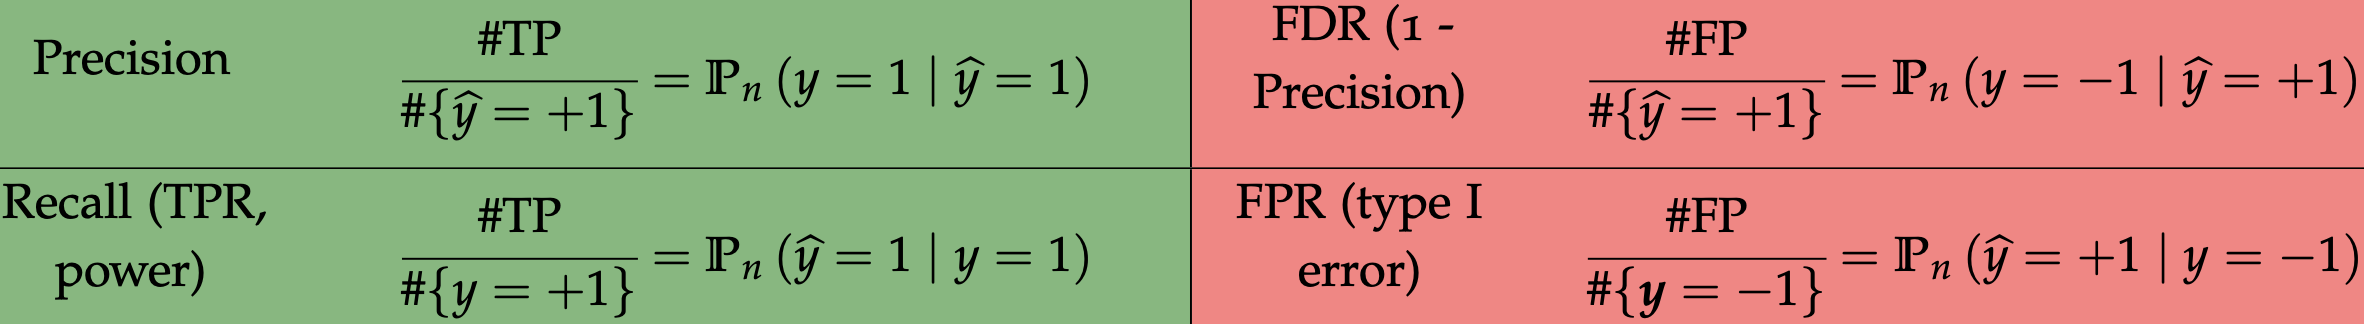
\includegraphics[width=0.495\textwidth]{Bilder/ClassificationTable.png}

% \vspace{3pt}

% Def: Sensitivity($\theta$) = TPR = $\mathrm{\frac{TP}{P}}$, Specificity($\theta$) = $\mathrm{\frac{TN}{N}}$, 1-sp($\theta$) = FPR = $\mathrm{\frac{FP}{N}}$.
% ROC Curve: Plot Sensitivity vs. 1-Specificity (TPR vs. FPR)

\vspace{-8pt}

\section{Flexible Regr. and Class. Methods}

\vspace{-5pt}

\subsection{Additive Models}
Model: $g_{add} (x) = \mu + \sum_{j=1}^p g_j (x_j)$ with $\mu \in \R$, $g_j : \R \rightarrow \R$, $\Expec [g_j (x_j)] = 0 \ \forall j=1,\dots,p$. $g_j$'s are non-parametric. Not affected by curse of dimensionality.

\vspace{5pt}

\fat{Backfitting}
Def: $S_j : (U_1,\dots,U_n)^T \mapsto (\hat{U}_1,\dots,\hat{U}_n)^T$. The index $j$ means the smoothing is done against the $j$-th predictor/parameter.

\fat{Algorithm}: 1) $\hat{\mu} := \frac{1}{n} \sum_{i=1}^n Y_i$ and $g_j (.) = 0$ $\forall j=1,\dots,p$

2) Cycle through indices: $j=1,\dots,p,1,\dots,p,1,\dots$ while computing: $\hat{\vec{g}}_j = S_j \klammer{\vec{Y} - \hat{\mu} \id - \sum_{k \neq j} \hat{\vec{g}}_k}$ where $\hat{\vec{g}}_j = (\hat{g}_j (X_{1j}),\dots,\hat{g}_j (X_{nj}))^T$ and stop if $\frac{\Norm{\hat{\vec{g}}_{j,new} - \hat{\vec{g}}_{j,old}}_2}{\Norm{\hat{\vec{g}}_{j,old}}_2} \leq \text{tol}$ (e.g. tol=$10^{-6}$)

3) Normalize: $\tilde{g}_j (.) = \hat{g}_j (.) - \frac{1}{n} \sum_{i=1}^n \hat{g}_j (X_{ij})$

\vspace{-5pt}

\subsection{Neural Networks}
Activation Functions: 1) Softmax: $\hat{\pi} \klammer{Y=k | \vec{X} = \vec{x}} = \frac{\exp (g_k (\vec{x}))}{\sum_j \exp(g_j(\vec{x}))}$ , 2) Sigmoid: $\phi(t) = \frac{e^t}{1+e^t} = \frac{1}{1+e^{-t}}$ , 3) ReLU: $\phi(t) = \max \geschwungeneklammer{0,t}$

\vspace{-5pt}

\subsection{Classification \& Regression Trees (CART)}
Model: $g_{tree} (\vec{x}) = \sum_{r=1}^M \beta_r \id_{[\vec{x} \in \mathcal{R}_r]}$ is a piecewise constant fct. with $\mathcal{P} = \mathcal{R}_1 \sqcup \dots \sqcup \mathcal{R}_M$ is a partition of $\R^p$.

\vspace{5pt}

\fat{Parameter Estimation} Regression and Binary Classification: $\hat{\beta}_r = \frac{\sum_{i=1}^n Y_i \id_{[\vec{x}_i \in \mathcal{R}_r]}}{\sum_{i=1}^n \id_{[\vec{x}_i \in \mathcal{R}_r]}}$ , $J$ Class Problem: $\hat{\beta}_r^{j} = \frac{\sum_{i=1}^n \id_{[Y_i =  j]} \id_{[\vec{x}_i \in \mathcal{R}_r]}}{\sum_{i=1}^n \id_{[\vec{x}_i \in \mathcal{R}_r]}}$

\vspace{5pt}

\fat{Search Algorithm} Restict partition $\mathcal{P}$ of $\R^p$ to axes parallel rectangles $\mathcal{R}_r$. 1) $M=1$, $\mathcal{P} = \geschwungeneklammer{\mathcal{R}} = \geschwungeneklammer{\R^p}$ , 2) Refine $\mathcal{R}$ into $\mathcal{R}_{left} \sqcup \mathcal{R}_{right}$ along one of the $p$ dimensions s.t. $-\log(\mathcal{L})$ is maximally reduced. Update $\mathcal{P} = \geschwungeneklammer{\mathcal{R}_1,\mathcal{R}_2} = \geschwungeneklammer{\mathcal{R}_{left},\mathcal{R}_{right}}$ , 3) Refine $\mathcal{P}$ by finding $\mathcal{R}_k$ and its split s.t. $-\log(\mathcal{L})$ is maximally reduced and update again: $\mathcal{P} = \mathcal{P}_{old} \backslash \R_{k} \cup \geschwungeneklammer{\mathcal{R}_{k,1},\mathcal{R}_{k,2}}$ , 4) Iterate step 3 for large nbr M , 5) Prune the tree until reasonable size.

\vspace{5pt}

\fat{Tree representation}
Select "best" tree by applying "cost complexity (=cp) pruning". Penalized goodness of fit: $R_\alpha (\tau) = R(\tau) + \alpha \cdot \text{size}(\tau)$. Here, size$(\tau)$ is the number of leaves in the tree $\tau$ and $R(.)$ is quality of fit measure. The \fat{best tree}: $\tau (\alpha) := \argmin_{\tau \subset \tau_M} R_{\alpha} (\tau)$. $\geschwungeneklammer{\tau(\alpha) | \alpha \in [0,\infty)}$ is a nested set and the same as the subsets of $\tau_M \supseteq \dots \supset \tau_{\emptyset}$. For model selection we need to select best $\alpha$ or its normalization $cp = \frac{\alpha}{R(\tau_{\emptyset})}$ using CV.

\vspace{5pt}

\fat{1SE Rule}
Take smallest tree s.t. its error is at msot one std error larger than the minimal one.

\vspace{5pt}

\fat{Pros and Cons}
\textcolor{red}{Greedy-tree-type altorithm produces unstable splits $\Rightarrow$ if one split is "wrong", everything below it will be "wrong".}

\vspace{-5pt}

\subsection{Random Forests}
\fat{Algorithm} 1) Draw $n_{tree}$ BS samples from original $\mathcal{D}$. 2) $\forall$ BS samples grow an unpruned classif./regr. tree (maybe use nodesize to lower bound the \#datapoints per node) s.t. at each node randomly sample $m_{try}$ of the pred. var. and chose best split from among these vars. 3) Pred. new data by aggregating predictions of the $n_{tree}$ trees (majority vote for classif. and average for regr.)

\vspace{5pt}

\fat{Remark} Bagging: $m_{try} = p$

\vspace{5pt}

\fat{Estimation of error} 1) At each BS iteration predict on OOB data. 2) Aggregate OOB pred. $\Rightarrow$ Calculate error rate


\vspace{-8pt}

\section{Reproducing Kernel Hilbert Spaces}

\vspace{-5pt}

\fat{Def (Kernel)} Let $\mathcal{X} \subseteq \R^d$. We call $k: \mathcal{X} \times \mathcal{X} \rightarrow \R$ a kernel iff $\forall m \ \forall x_1,\dots,x_m \in \mathcal{X}: \ K \in \R^{m \times m}$ with $K_{ij} := k(x_i,x_j)$ is psd and symm. (psd: $\forall c \in \R^m: c^T K c \geq 0$, symm: $\forall x,y \in \mathcal{X}: \ k(x,y) = k(y,x)$)

\vspace{5pt}

\fat{Def (RKHS)} Let $\mathcal{H}$ be a hilbert space of fcts $f: \mathcal{X} \rightarrow \R$. $\mathcal{H}$ is a Reproducing Kernel Hilbert Space (RKHS) iff $\exists k : \mathcal{X} \times \mathcal{X} \rightarrow \R$ s.t. $\forall x \in \mathcal{X}: k(x,.) \in \mathcal{H}$ and $\forall f \in \mathcal{H} \forall x \in \mathcal{X}: \scalprod{f(.)}{k(x,.)} = f(x)$

\vspace{5pt}

\fat{Median Heuristic}
Gaussian kernel: $2 \sigma^2 = \text{median} \klammer{\Norm{x_i - x_j}^2}_{i \neq j}$

\vspace{-13pt}

\subsection{Support Vector Machines (SVM)}
Assume $\mathcal{D}$ is linearly seperable. Goal: separate $\mathcal{D}$ into two classes with a hyperplane: find $w \in \R^d$ and $b \in \R$ s.t. $\min_{i \in \geschwungeneklammer{1,\dots,n}} \abs{\scalprod{w}{x_i} + b} = 1$ (canonical form). The distance of the hyperplane to the closest $x_i$ is called the \fat{margin}. If in canonical form: margin$=\frac{1}{\Norm{w}_2}$.

\vspace{5pt}

\fat{Algorithm} \textcolor{blue}{Soft}/\textcolor{purple}{Hard} SVM:
$\textcolor{purple}{\min_{w,b} \frac{1}{2} \Norm{w}_2^2} \textcolor{blue}{+ c \cdot \sum_{i=1}^n \xi_i}$ s.t. $\textcolor{purple}{\forall i \in \geschwungeneklammer{1,\dots,n} \ y_i \klammer{\scalprod{w}{x_i} + b} \geq 1} \textcolor{blue}{-\xi_i}$.


\vspace{-8pt}

\section{Bagging \& Boosting}

\vspace{-5pt}

\subsection{Bagging}
Consider a tree algorithm yielding $\hat{g}(.): \R^p \rightarrow \R$.

\vspace{5pt}

\fat{Algorithm} 1) Generate BS samples: $(X_1^*,Y_1^*),\dots,(X_n^*,Y_n^*)$ and compute $\hat{g}^* (.)$. 2) Repeat 1 B times: $\hat{g}^{*1} (.), \dots, \hat{g}^{*B} (.)$. 3) Aggregate: $\hat{g}_{Bag} (.) = \frac{1}{B}\sum_{i=1}^B \hat{g}^{*i} (.) \approx \Expec^* \eckigeklammer{\hat{g}}^*(.)$

\vspace{5pt}

\fat{Remark} $\Expec \eckigeklammer{\klammer{Y-\hat{f}_{Bag}(X)}^2} \leq \Expec \eckigeklammer{\klammer{Y-\hat{f}^* (X)}^2} = \Expec \eckigeklammer{\klammer{Y-\hat{f}_{Bag}(X)}^2} + \underbrace{\Expec \eckigeklammer{\klammer{\hat{f}_{Bag} (X) - f^* (X)}^2}}_{=Var(f^* (X))}$

\vspace{5pt}

\fat{Bagging for trees}
Setup: Regr.Trees s.t. exactly $m$ training samples are in each leaf node. Model: $\hat{Y}(x) = \sum_{i=1}^n w_i Y_i$ where $w_i = \frac{1}{m} \id_{\geschwungeneklammer{x_i \& x \ \text{in same leaf}}}$. Hence: $\hat{Y}_{Bag} (x) = \sum_{i=1}^n \klammer{\frac{1}{B} \sum_{b=1}^B w_i^{*b}} Y_i = \sum_{i=1}^n w_{bag,i} Y_i$ where $w_i^{*b} \in \geschwungeneklammer{0,\frac{1}{m}}$.

\vspace{5pt}

\fat{Remark} $\Var \klammer{\hat{Y}_{bag} (X)} = \sigma^2 \sum_{i=1}^m w_{bag,i}^2 \leq \sigma^2 \sum_{i=1}^m w_i^2 = \Var \klammer{\hat{Y}(x)}$ Hence Bagging is a Variance reducing technique.

\vspace{-5pt}

\subsection{Boosting}
Boosting is a bias reducing technique.

\vspace{5pt}

\fat{AdaBoost} $g: \R^p \rightarrow \geschwungeneklammer{-1,1}$, $Y \in \geschwungeneklammer{-1,1}$, Idea: upweight observations previous model got wrong.

1) Initialize obs. weights $w_i = \frac{1}{N} \ \forall i=1,\dots,N$

2) For $m=1,\dots,M$: a) Fit classifier $\hat{g}_m (.)$ using $w_i$, b) Compute weighted error: $err_m = \frac{\sum_{i=1}^N w_i \id_{\geschwungeneklammer{Y_i \neq \hat{g}_m (x_i)}}}{\sum_{i=1}^N w_i}$, c) Compute $\alpha
_m = \log \klammer{\frac{1-err_m}{err_m}}$, d) Set weights: $w_i = w_i \cdot \exp \klammer{\alpha_m \cdot \id_{\geschwungeneklammer{Y_i \neq \hat{g}_m (x_i)}}}$

3) Final Model: $\hat{G} (x) = \sign \klammer{\sum_{m=1}^M \alpha_m \hat{g}_m (x)}$

\vspace{5pt}

\fat{Gradient Boosting}
Goal: $G(x) = g_0 (x) + \sum_{m=1}^M \gamma \cdot g_m(x)$

1) Initialize $G(x) = g_0 (x)$

2) For $m=1,\dots,M$: a) $\forall i=1,\dots,N$: $r_{im} = - \frac{\partial \mathcal{L} (y_i,G(x_i))}{\partial G(x_i)}$, b) fit Model $g_m (x_i)$ to $r_{im}$, c) set $G(x) = G(X) + \gamma g_m(x)$ for $\gamma \in (0,1]$


\vspace{-8pt}

\section{Random Additional Material}

\fat{Cook's Distance:} Measure of Influence of a datapoint. $D_i := \frac{\sum_{j \neq i}\klammer{\hat{Y}_j - \hat{Y}_j^{-i}}^2}{p \cdot \Norm{Y - \hat{Y}}^2 / (n-p)}$, $\hat{Y}_j^{-i}$ is the fitted value of $j$ when disregarding point $i$ during fitting. $D_i>0$ means $x_i$ is very influential.

\vspace{-8pt}

\section{R Code}

\vspace{-5pt}

%\subsection{Useful Functions}

\begin{tabularx}{0.495\textwidth} {l|X}
    \hline
    Function & Description \\ \hline
    \texttt{solve()} & invert Matrix \\
    \texttt{t()} & transpose Matrix \\
    \texttt{\%*\%} & matrix multiplication \\
    \texttt{df[,-c(6)]} & remove column 6 from df \\
    \texttt{seq(1,40,1)} & generate sequence of evenly spaced values \\
    \texttt{rep(1,7)} & create a ones-vector of length 7 \\
    \texttt{rnorm(n)} & generate $n$ random numbers based on normal distr \\
    \texttt{rgamma()} & generate random numbers based on gamma distr \\
    \texttt{factor()} & apply to a vector if it is categorical to be able to perform regression tasks \\
    \texttt{which.max()} & returns index of maximal entry in a vector (/matrix) \\
    \texttt{as.formula()} & takes a text ("y$\sim$.") as input and stores it as a formula \\
    \texttt{scale(mat)} & center and scale columns of a matrix / df \\
    \texttt{fitted(fit)} & returns fitted values of a model \\
    \texttt{resid(fit)} & returns residuals of a model \\
    \texttt{boxplot(a[])} & creates boxplot of vector a \\
    \texttt{quantile(...)} & $x$=data, probs$=$0.75 (e.g.): computes 75\% quantile of x \\
    \texttt{predict(...)} & args: \texttt{fit} (fitted model), \texttt{type}: e.g. \texttt{"response"} \\
    \texttt{gam()} & package \texttt{mgcv}; generalized additive model. Used for adaptive models: e.g. smoothing-spline for log reg \\
    \texttt{nnet()} & fits a feedforward NN \\
    \texttt{ppr()} & projection pursuit regression (extension of additive models) \\
    \texttt{rpart()} & package \texttt{rpart}; used for fitting classification and regressino trees; \texttt{type="class"} if classification tree \\
    \texttt{sd()} & compute standard deviation \\
    \texttt{glm} & package \texttt{glmnet}; generalized linear models (e.g. linear logistic regression) \\
\end{tabularx}

\begin{tabularx}{0.495\textwidth} {l|X}
    \hline
    Function & Description \\ \hline
    \texttt{optim()} & can maximize/minimize a function \\
    \texttt{choose(n,k)} & Binom Coeff \\
    \texttt{plotcp()} & choose optimal tree pruning parameters (also \texttt{plotcp()}) \\
    \texttt{prune.rpart()} & do pruning on tree \\
    \texttt{density()} & density distribution; use \texttt{bw="SJ"} to get iteratively found optimal bandwidth \\
    \texttt{ksmooth()} & Nadaraya-Watson kernel regression estimate; Returns Vector \\
    \texttt{smooth.spline()} & smooth spline estimator \\
    \texttt{loess()} & local polynomial regression \\
    \texttt{boot.ci()} & \texttt{boot.ci(boot.out=res.boot,conf=0.95,} \\
     & \texttt{type=c("basic","norm","perc"))} computes the reversed, normal approx. and quantile-quantile of the bootstrap \\
    \texttt{coefficients()} & get coefficients of a fit, (e.g. \texttt{reg <- lm(y~x)} and then \texttt{coefficients(reg)[2]}) \\
    \texttt{pairs()} & make a pair-plot \\
    \texttt{\$sigma} & e.g. \texttt{summary(fit5)\$sigma} \\
    \texttt{prp()} & plot a tree \\
    \texttt{svm} & Kernel SVM \\
    \texttt{med.heur <- } & \texttt{1/median(dist(iris[samp,1:4])$\wedge$2)} \\
    \texttt{multinom} & (e.g. \texttt{multinom(Species~.,data=Iris)}) Multinomial regression
\end{tabularx}

\vspace{-5pt}

% \subsection{Code Examples}

% \vspace{-14pt}

\begin{lstlisting}[style=RStyle, caption={Theoretical True distribution},numbers=none]
X <- cbind(1, x)                ## design matrix
XtXinv <- solve(crossprod(X))   ## theoretical s.d.
tsd <- sqrt(5^2*XtXinv[2,2])
\end{lstlisting}

\vspace{-14pt}

\begin{lstlisting}[style=RStyle, caption={Backward/Forward Selection},numbers=none]
mortal.full <- lm(Mortality~.,data=mortality)
mortal.empty <- lm(Mortality~1,data=mortality)
mortal.bw <- step(mortal.full,dir="backward")
mortal.fw <- step(mortal.empty,dir="forward",scope=list(upper=mortal.full,lower=mortal.empty))
library(leaps)
mortal.alls <- regsubsets(Mortality~.,data=mortality)
p.regsubsets(mortal.alls,cex=0.8,cex.main=.8)
\end{lstlisting}

\vspace{-14pt}

\begin{lstlisting}[style=RStyle, caption={Non-parametric Regression},numbers=none]
bmwloess <- loess(y~x)      # local polynomial
dgf <- bmwloess$trace.hat   # degrees of freedom
bmwss <- smooth.spline(x,y,df=dgf)  # smooth spline
ox <- order(x)              # k-smooth destroyes order
bmwks <- ksmooth(x,y,kernel="normal",bandwidth=h,x.points=x) # Nadaraye-Watson
bmwks$x <- bmwks$x[order(ox)]
bmwks$y <- bmwks$y[order(ox)]
plot(x,y)
lines(x_new,bmwks$y)
lines(x_new,predict(bmwloess,newdata=data.frame(x=x_new)))
llines(x_new,predict(bmwss,x=x_new)$y)
\end{lstlisting}

% \vspace{-14pt}

% \begin{lstlisting}[style=RStyle, caption={ANOVA},numbers=none]
% fitfull<-lm(thorax~v1+v2+v3+v4)
% fitintercept<-lm(thorax~1)
% anova(fitintercept,fitfull)

% fit_gFull <- lm((longevity) ~ thorax + dummy.1.p + dummy.1.v + dummy.8.p + dummy.8.v)
% fit_gPart <- lm((longevity) ~ thorax + I(dummy.1.v + dummy.1.p) + I(dummy.8.p + dummy.1.p) + I(dummy.8.v - dummy.1.p))
% anova(fit_gPart,fit_gFull)
% \end{lstlisting}

\vspace{-14pt}

\begin{lstlisting}[style=RStyle, caption={Hat Matrix},numbers=none]
Snw <- Slp <- Sss <- matrix(0, nrow = n, ncol = n)
## The j-th column is given by S_j = Snw[,j]
In <- diag(n)
for(j in 1:n) {
    Snw[,j] <- ksmooth(x, In[,j], kernel = "normal", bandwidth = 0.2,x.points = x)$y
}
df.NW <- sum(diag(Snw))
## Getting the span parameter for loess and spar parameter for smooth.spline such that the degrees of freedom are (approximately) the same with the ones for Nadaraya-Watson estimator
dflp <- function(span, val) {
    for(j in 1:n)
        Slp[,j] <- loess(In[,j] ~ x, span = span)$fitted
    sum(diag(Slp)) - val
}
span <- uniroot(dflp, c(0.2, 0.5), val = df.NW)$root
for(j in 1:n) {
    Slp[,j] <- predict(loess(In[,j] ~ x, span = span), newdata = x)
    Sss[,j] <- predict(smooth.spline(x, In[,j], df = df.NW), x = x)$y
}
spar <- smooth.spline(x, In[,1], df = df.NW)$spar
...
estnw[,i] <- ksmooth(x, y, kernel = "normal", bandwidth = 0.2, x.points = x)$y
sigmanw <- sum((y - estnw[,i])^2) / (length(y) - sum(diag(Snw)))
senw[,i] <- sqrt(sigmanw * diag(Snw %*% t(Snw)))
...
\end{lstlisting}

\vspace{-14pt}

\begin{lstlisting}[style=RStyle, caption={Coverage Function},numbers=none]
coverage <- function(x,est,se) {
    pos <- x == 0.5
    pw <- sum(abs(est[pos,] - m(x)[pos]) <= 1.96*se[pos,]) # pointwise coverate
    simult <- sum(apply(abs(est - m(x)) <= 1.96 * se, 2, all)) # simultaneous coverage }
\end{lstlisting}

\vspace{-14pt}

\begin{lstlisting}[style=RStyle, caption={Confidence Intervals},numbers=none]
newcountry <- data.frame(l2tv=log2(50),l2dr=log2(3000))
predict(fit,newdata=newcountry,interval="confidence")
\end{lstlisting}

\vspace{-14pt}

\begin{lstlisting}[style=RStyle, caption={LOOCV},numbers=none]
loocv <- function(reg.data, reg.fcn){
    loo.reg.value <- function(i, reg.data, reg.fcn)
        return(reg.fcn(reg.data$x[-i], reg.data$y[-i], reg.data$x[i]))
    n <- nrow(reg.data)
    loo.values <- sapply(1:n, loo.reg.value, reg.data, reg.fcn)
    mean((reg.data$y - loo.values)^2)
}
\end{lstlisting}

\vspace{-14pt}

\begin{lstlisting}[style=RStyle, caption={CV},numbers=none]
h <- 4
reg.fcn.nw <- function(reg.x, reg.y, x)
    ksmooth(reg.x, reg.y, x.points = x, kernel = "normal", bandwidth = h)$y
(cv.nw <- loocv(reg, reg.fcn.nw))
n <- nrow(reg)
Id <- diag(n)
S.nw <- matrix(0, n, n)
for (j in 1:n)
    S.nw[, j] <- reg.fcn.nw(reg$x, Id[, j], reg$x)
(df.nw <- sum(diag(S.nw)))
y.fit.nw <- reg.fcn.nw(reg$x, reg$y, reg$x)
(cv.nw.hat <- mean(((reg$y - y.fit.nw)/(1 - diag(S.nw)))^2))
library(sfsmisc)
hatMat(reg$x,trace=TRUE,pred.sm=reg.fcn.nw,x=reg$x)
S.nw.hatMat <- hatMat(reg$x,trace=FALSE,pred.sm=reg.fcn.nw,x=reg$x)
(cv.nw.hatMat <- mean(((reg$y - y.fit.nw)/(1 - diag(S.nw.hatMat)))^2))
...
est.ssopt <- smooth.spline(reg$x, reg$y, cv = TRUE)
cv.ssopt <- est.ssopt$cv.crit
\end{lstlisting}

\vspace{-14pt}

\begin{lstlisting}[style=RStyle, caption={Bootstrapping},numbers=none]
tIQR <- function(x, ind) IQR(x[ind])
require("boot")
res.boot <- boot(data = sample40, statistic = tIQR, R = 10000) # sim="ordinary"
bci <- boot.ci(res.boot, conf = 0.95, type = c("basic", "norm", "perc"))
\end{lstlisting}

\vspace{-14pt}

\begin{lstlisting}[style=RStyle, caption={LDA, QDA, logistic regression and ROC Curve},numbers=none]
class_lda <- lda(x = Iris[, c("Petal.Length", "Petal.Width")], grouping = Iris[, "Species"])
predplot(class_lda, Iris, main = "Cl. w/ LDA")
class_qda <- qda(x = Iris[ ,c("Petal.Length", "Petal.Width")],grouping = Iris[, "Species"])
predplot(class_qda, Iris, main = "Cl. w/ QDA")
## Use function multinom to fit data
class_multinom <- multinom(Species ~ . , data = Iris)

require(ROCR)
fit <- glm(Survival ~ ., data = d.baby, family = "binomial")
pred <- prediction(fit$fitted.values, d.baby$Survival)
perf <- performance( pred, "tpr", "fpr" )
plot(perf, main = "ROC")
perf.cost <- performance(pred, "cost")
plot(perf.cost, main = title)
\end{lstlisting}

\vspace{-14pt}

\begin{lstlisting}[style=RStyle, caption={GAMs},numbers=none]
require(sfsmisc)
form5 <- wrapFormula(logupo3~., data = d.ozone.e, wrapString="poly(*,degree=5)")
fit5 <- lm(form5, data = d.ozone.e)
require(mgcv)
gamForm <- wrapFormula(logupo3~., data = d.ozone.e)
g1 <- gam(gamForm, data = d.ozone.e)
# Formula: logupo3 ~ s(vdht) + s(wdsp) + s(hmdt) + s(sbtp) + s(ibht) + s(dgpg) + s(ibtp) + s(vsty) + s(day)
\end{lstlisting}

\vspace{-14pt}

\begin{lstlisting}[style=RStyle, caption={Trees and Forests},numbers=none]
rp.veh0 <- rpart(Class~.,data=d.vehicle,control=rpart.control(cp=0.0,minsplit=2))
preds = predict(rp.veh0,newdata=d.vehicle,type="class")
table(d.vehicle$Class, preds)
cp.opt <- rp.veh$cptable[7, "CP"]
rp.veh.pruned <- prune.rpart(rp.veh, cp = cp.opt)
library(randomForest)
rf.model1 <-randomForest(factor(Class)~.,data=d.vehicle)
\end{lstlisting}

\vspace{-14pt}

\begin{lstlisting}[style=RStyle, caption={Ridge and Lasso},numbers=none]
require(glmnet)
f.ridge <- glmnet(X, Y, alpha=0)
f.lasso <- glmnet(X, Y, alpha=1)
cv.eln <- cv.glmnet(X, Y, alpha=0.5, nfolds=10)
lambda.min <- cv.eln$lambda.min
lambda.1se <- cv.eln$lambda.1se
plot(log(f.lasso$lambda),apply(coef(f.lasso), 2, function(x) sum(x != 0)), type = "l", ylab = "Nbr selected preds") # could also use f.lasso$beta for apply(...)
first.lam.ind = min(which(f.lasso$df >= 16))
# coef(f.lasso)[, first.lam.ind] gets coeffs for this lambda
names(which(coef(f.lasso)[, first.lam.ind] != 0))
\end{lstlisting}


\end{document}